\section{Versuchsaufbau/-durchführung}

\subsection{Bestimmung der Durchlasskurve für den $LC$- und $LC_1 C_2$ Kette}
Zunächst wird der Aufbau, wie in Abbildung \ref{fig:aufbau_durchlass} zusehen aufgebaut. %überarbeite diesen satz nochmal
\begin{figure}
  \centering
  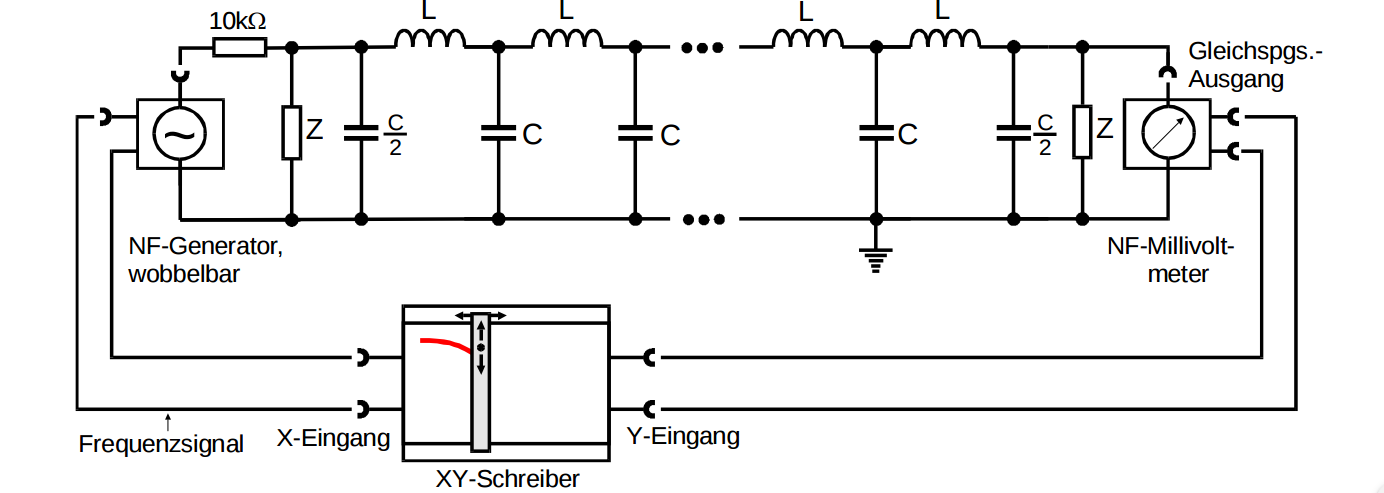
\includegraphics[width=0.8\textwidth]{bilder/versuchsaufbau_1.png}
  \caption{Versuchsaufbau für die bestimmung der Durchlasskurve}
  \label{fig:aufbau_durchlass}
\end{figure}

Zu Beginn wird an dem NF-Generator ein Frequenz Sweep eingestellt.
In dem Frequenzbereich des Sweeps muss die Grenzfrequenz liegen, bei der die
Kettenschaltung Strom undurchlässig wird. %stromundurchlässig
Am Kettenanfang und -ende werden die Widerstände $Z$ auf den theoretisch
berechneten Wellenwiderstand eingestellt.
Die am Kettenende anliegende Spannung und die vom Generator ausgegebenen Frequenzen
werden an einem XY-Schreiber gegeneinander aufgetragen.
Wichtig dabei ist, dass zu beliebig ausgewählten Punkten, die gerade anliegende Frequenz bekannt ist. %Hier noch mehr dazu ? %sag einfach, dass 6 referenzpunkte aufgenommen wurden


\subsection{Bestimmung der Dispersionskurve}
Der Versuch wird wie in Abbildung \ref{fig:aufbau_dispersion} zusehen ist, aufgebaut. %überarbeite diesen satz nochmal
\begin{figure}
  \centering
  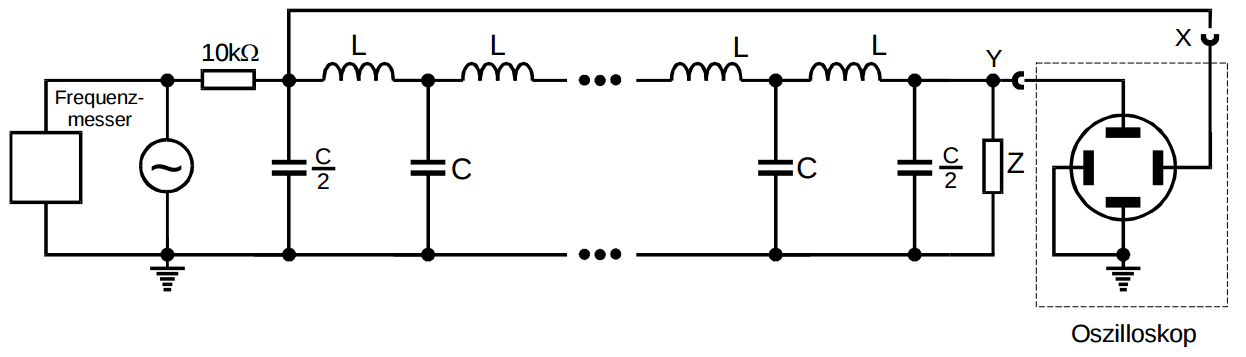
\includegraphics[width=0.8\textwidth]{bilder/versuchsaufbau_dispersion.png}
  \caption{Versuchsaufbau für die Messung der Dispersionskurve}
  \label{fig:aufbau_dispersion}
\end{figure}

Anschließend werden für die verwendeten $L$, $C_1$ und $C_2$ die Wellenwiderstände berechnet %für die verwendeten Bauteile
und die An- und Abschlusswiderstände $Z$ auf diesen Wert eingestellt.
Mithilfe von Lissajou-Figuren werden nun die Frequenzen bestimmt, wo eine Phasenverschiebung von $\pi$ %'wo' umgangssprachlich
vorhanden ist. Anschließend kann dann mit der Anzahl der Kettenglieder auf die, %-komma
Phasenverschiebung pro Kettengleid geschlossen werden.

\subsection{Ausmessung der stehende Welle}
Der Versuch wird nach Abb. \ref{fig:aufbau_dispersion} aufgebaut.
Nun wird einmal mit und einmal ohne Wellenwiederstand $Z$, die Spannung einem Millivoltmeter gemessen. %überarbeite diesen satz nochmal
Zunächst wird die Spannung am Kettenanfang abgegriffen, um so ein frequenzabhängiges Spannungsmaximum
zufinden. Für die ersten beiden Maxima werden bei allen Kettengliedern die anliegende Spannung gemessen. % zu finden
Für die restlichen Maxima werden nur die dazugehörigen Frequenzen notiert.
